\section{LBox: a User-level Logging Framework for Linux}

\subsection{Introduction and Overview}

Logging and auditing are important operating system facilities used
to help monitor correct system operation and to detect potential
security problems.
In Unix systems, logging is traditionally {\em application based}.
The application itself controls what is being logged through
the system logging mechanism \code{syslog}, e.g.
security audit log messages generated 
by \code{login}, \code{su}, etc.
The drawback of application logging is since it is under the
control of an application which may be compromised or malicious,
no security guarantees are possible.
More secure versions of Unix have finer grained auditing mechanisms
to satisfy the Trusted Computer System Evaluation Criteria (TCSEC) or Common
Criteria (CC) security requirements.
The Solaris Basic Security Module \cite{solaris-sec-svc}
for example defines kernel auditing events 
which can serve to log certain system calls.
Such auditing is typically system-wide on all processes and
requires administrator privileges.

Traditional auditing mechanisms are designed mainly for
system audit trail purposes.
As such, they are not sufficient for the needs
of more demanding security monitoring applications
such as intrusion detection systems (IDS), 
determining correct application behavior, detecting improper system usage, etc.
In this paper, we present an approach to auditing and monitoring
which is sufficiently flexible for a variety of applications.
We provide a kernel extension which enables easy
programming of user level (as opposed to kernel level) monitors for 
observing the effects of system calls made by specified processes of interest.
Our philosophy is to separate mechanism from policy.
A kernel-level mechanism provides transparent, secure and efficient monitoring,
while the core logic and functionality is encapsulated in a user-level monitor.
Having a user-space monitor means that
we do not have to worry about code safety
issues unlike a kernel-level one.
As user-level monitors do not have to be privileged, 
ordinary users can create/run their own monitoring tools.
We show that general purpose user-level monitors are easy to write 
without requiring any knowledge of kernel programming. 
In the remainder of this paper, we will refer to monitoring as encompassing
the concept of auditing and logging.

We provide a number of security guarantees:
(i) the selected processes (which can include their children)
cannot circumvent monitoring, we call this {\em mandatory monitoring};
(ii) none of the operations/events of interest from the set of monitored
processes are missed, we call this {\em reliable monitoring};
and 
(iii) the monitor cannot escalate its privileges, only precisely
the operations/events of processes at the same privilege level can
be monitored.
The mandatory and reliable properties are necessary to ensure that a monitor
can be used for security purposes.
The last property is important since the user-level monitors can be 
unprivileged.
Finally we also require that the monitor be {\em transparent} to the monitored
processes --- thus the act of being monitored has no side effects to the
monitorees.
We remark that traditional Unix mechanisms such as \code{ptrace} and 
\code{proc} do not provide these guarantees.

A key objective is that the monitoring mechanism be efficient and scalable.
By efficiency, we mean that fine-grained monitoring is possible with low
overheads.
Scalability means that the cost of monitoring should be dependent on
how much is being monitored and the amount of information desired.
The cost should be controllable by the monitor so that overhead is
commensurate with need.
In the end, we want to be able to have several fine-grained root-level and 
unprivileged monitors to be permanently running without 
paying too high a price. 
On one end of the spectrum, we allow for global monitors which
log all interesting events across all processes to disk like 
an audit log; and on the other end, the monitor might only be concerned
with writes to particular system files from particular processes
and then perform sophisticated analysis.
% An efficient mechanism is also needed to avoid the impact of denial of
% service attacks, i.e. a disk (or remote) log is constrained 
% by the bandwidth of I/O.

Consider the following motivating example.
Suppose we want to monitor whether a web server has been attacked,
perhaps as part of an IDS.
The web server logs cannot be used since either
the server or the logs could be compromised. 
A traditional auditing facility like a disk based log would 
have a number of problems. Firstly, there may be confidentiality
issues in giving the system log to the IDS, the IDS may gain access to
confidential information (assuming it isn't running as root).
Another question is what happens if the disk log 
causes the filesystem to run out of space?
Add a network IDS to this scenario will further strain the audit log!
One could use \code{ptrace} to monitor the web server 
but this can have a significant performance penalty and may
not ensure mandatory or reliable auditing.

Our prototype implementation shows that it is possible to to get all
these desirable features in a user-space monitor without requiring special
privileges. Furthermore, we demonstrate an efficient implementation
which has low overhead even though the monitors are in user-space.

\subsection{Related Work and Approaches}

A commonly used technique for monitoring is system call tracing or system call
interposition to monitor the system calls made by a process.
For portability, systems like Janus \cite{janus} or Alcatraz \cite{alcatraz}
use the Unix user-level mechanisms \code{ptrace} or \code{proc} to do
system call tracing.
This usage is problematic because it is not
meant to be a secure monitoring mechanism, e.g.
\code{ptrace} was meant to support debuggers.
In the Solaris manual pages, \code{ptrace} is described as being
``unique and arcane''.
\cite{garfinkel} discuss 
these kinds of problems and common
pitfalls with user-level system call interposition
are discussed in \cite{garfinkel}, such as:
(i) race conditions between time of check and time of use (TOCTOU), 
i.e. a buffer can be modified by another thread;
(ii) non-inheritance of tracing, i.e. special \code{strace} hacks in Linux;
and (iii) not transparent with respect to setuid/setgid executables 
and signals,
i.e. \code{ptrace} and \code{proc} disable tracing 
on setuid/setgid executables.  
Because of their subtleties and intrinsic difficulties,
\code{ptrace} or \code{proc} are not suitable for general purpose user-level
monitoring although they may be useful in specific situations.\footnote{
We remark that a simple program can cause both
\code{strace} in Linux and \code{truss} in Solaris to misbehave.
}

The other serious drawback of \code{ptrace} or \code{proc} is that
the overhead is considerable, incurring at least two
context switches per traced system call.
Our micro benchmarks show that this can lead to an order of magnitude
slowdown on system call intensive programs.
Another example is Alcatraz \cite{alcatraz},
their user-level system call interception mechanism gives an overhead of 77\%
on a \code{tar} benchmark.
Thus, user-level mechanisms also have the drawback
of high intrinsic overhead.

The obvious alternative is a kernel-level system call interposition,
e.g. the later version of Janus used a kernel module, \code{mod\_janus}
\cite{garfinkel}.
We remark that while a kernel-level system call interposition
is more efficient and can be transparent, one still has to be
careful about race conditions.
For example, Systrace \cite{systrace} takes special care to address aliasing
and atomicity.

Efficient user-level monitoring also however requires a 
flexible mechanism to reduce the overhead of communication and
the number of context switches to the user-level monitor, so this is more
than what is done in system call interposition.
To further improve efficiency, we provide specifications which
can be checked more efficiently than a general purpose argument analysis
as in system call interposition.

Systems such as Janus and Systrace are intended for sandboxing or
confinement.
For example, Systrace uses a user-level policy daemon which implements the
confinement policy. 
Efficiency is obtained by implementing some of
the policy in the kernel and having a timely mechanism to invoke
the user-level daemon for the other cases.
Monitoring for auditing is different from confinement in that confinement
uses synchronous events while auditing uses asynchronous events.
Furthermore for auditing, we want to 
efficiently monitor large numbers of relevant events
and have minimal system impact on those events which are
not relevant.
The scope of processes being monitored may be quite different.
We can monitor a collection of processes which
do not form a proper subtree in the process hierarchy sense,
whereas a sandbox monitors processes which form a subtree.
We also provide a choice between reliable monitoring (no events are missed)
and unreliable monitoring (some events are allowed to be missed).

Systems for instrumenting and tracing the kernel can also capture
data similar to the ones which we are auditing.
% We remark that such systems are typically meant for debugging and
% analyzing system performance rather than for auditing and security purposes.
The most interesting one is the new
Dynamic Tracing (DTrace) facility \cite{dtrace-paper}
in Solaris 10.
DTrace allows almost all aspects of the kernel to
be instrumented, with 30,000 probes in the kernel.
DTrace uses a scripting language, D programs,
which are run within the kernel to do monitoring.
DTrace is extremely powerful because 
they run within the kernel and also because of the large number of
instrumented probes.
In-kernel also means that DTrace can be efficient.\footnote{
However, our micro-benchmarks indicate that while it is significantly
faster than \code{proc}, we have observed a factor of 2x slowdown.
}
To ensure safety of running in the kernel, DTrace programs
are restricted and checked for safety.
However, we believe that it is far safer to run monitors in user mode.

As kernel tracing mechanisms are meant for debugging and performance analysis,
they differ from monitors for auditing.
For example, although DTrace does integrate in privileges,
it does not have the same security concerns.
As kernel tracing is meant to minimise impact, DTrace does not provide
reliable event monitoring and can drop events.
Another difference with our framework is the auditing of file operations.
Since logging access to files is a very important for many kinds of monitoring,
we provide more powerful specifications on directories and subtrees.
The DTrace implementation requires extensive changes to Solaris, 
in the words of the developers, 
``it was a hell of a lot of work -- Bryan Cantrill, Solaris
Kernel Development''.
While it is difficult to have portable kernel enhancements, we feel our
approach is less of a massive change to the kernel type solution and in
this sense is more lightweight and amenable to implementation 
in different Unixes.

% Our approach differs from system call interposition mechanisms like
% {\tt ptrace()} and the syscall provider in {\tt DTrace} in that like the Linux
% Security Module (LSM) architecture \cite{lsm} -- we monitor access to objects
% rather than the system calls. For example, this makes it much easier to
% monitor files. We also have a rather different security 
% mechanism than {\tt DTrace}
% and no special privileges are required to be able to perform monitoring.
% We have a flexible mechanism to allow non-privileged monitors to only
% monitor selected events.


\subsection{The Monitor Framework}
\label{sec:framework}

A monitor is a user-space process which audits the behavior of other processes.
Monitors are described by two specifications:
(a) a process specification defining which processes to monitor; and
(b) event specifications which define what operations to monitor from
those processes.
In what follows, we describe the design of our monitoring framework and
portions of the API. The API is actually a user library which provides
a convenient interface to the kernel monitoring interface.
Due to lack of space, we will cannot give all the underlying
details but rather illustrate by example.

\subsubsection{The Monitor Process Specification}

An arbitrary collection of processes, not necessarily related by parent-child
relationships can be designated for mandatory monitoring.
To allow for flexibility and dynamic process creation (including children),
we use an API for constructing boolean expression in a functional lisp-like
style which allows easy creation in C.
The boolean expression is built from the following predicates using
the following usual boolean operators, \code{AND}, \code{OR} and \code{NOT}:

\begin{enumerate}

\item {\em true/false}:
For example, a global specification to monitor all
processes is simply the boolean expression {\em true}.

\item {\em uid/euid/suid/fsuid} (user id):
These predicates are true if and only if the
user id of the process is same as the user id specified.
Similar predicates are also used for group ids.

\item {\em pid} (process id):
This predicate is true if and only if the pid of the process
is same as the pid specified.
This is used to include or exclude existing processes.

\item {\em childof}:
This predicate is true if and only if the process specified by the pid
is an ancestor of the current process.
Note that we do not distinguish direct child processes
and grandchild processes - so childof can specify a subtree in the
process hierarchy.
This can be used to include or exclude both existing processes and processes
which are not yet created.

\item {\em executable}:
This predicate is true 
when the executable of the process is the same as the given pathname.
This can be used to include or exclude both existing processes and processes
which are not yet created.

\end{enumerate}

% An example of the use of process and event specification
% is the simple monitor given in Figure \ref{eg-prog} from Section \ref{sec-eg}.
% By using boolean expression, process specification can be very flexible.
\noindent
An example of the API (see also Section \ref{sec-eg}) is to monitor
all processes owned by the user Bob
except for process 1468 and its child processes.
{\small
\begin{verbatim}
  proc_spec = lbox_AND(
   lbox_UID("bob"),
   lbox_NOT(
     lbox_CHILDOF(1468)));
\end{verbatim}
}
Thus, the monitor can be targeted to observe only the activities
of particular processes of interest, ignoring other processes. 
This helps to reduce monitoring overhead.

\subsubsection{The Event Specification List}

An event specification defines which behaviors
of the monitored processes is of interest to the monitor.
Suppose a monitor event expression is $S$
and event $e$ happens. Then $S$ is triggered when $e$ is an object 
which matches $S$ and the operation is one which is compatible with $S$.
The notion of matching and compatibility is specific to the type of object.

A monitor defines a list of all the events of interest.
The event specification also defines the appropriate
information to return when an event is triggered.
One monitor might specify that a file event should 
consist of the inode, canonical pathname and operation type.
Another monitor might only need the operation type, perhaps because
the file is unambiguous and known to the monitor.
This helps achieve scalability. In the previous example,
it avoids the need for constructing a canonical
pathname and reduces the event size.

Our events are specified on system resources or objects together with their
associated operations. 
We feel this is more declarative than a system call approach
and makes it easier to specify the events of interest.
Due to lack of space, we will focus on file objects and briefly mention
other important system objects.
Common information which can be specified
for all types of events are:
\begin{enumerate}
\item {\em time}:
This gives the wall clock time of the event.
% Time is expressed in Linux clock ticks (jiffies). 
% It can be translated into human readable
% time format by the library we provide.
\item {\em pid}:
This is the process which performs the operation.
\item {\em type}:
The operation type which is specific to the object.
\end{enumerate}

All event specifications can 
specify whether the event is asynchronous and can be buffered up,
or if it is synchronous and needs to be delivered directly to the monitor.
Synchronous events also flush any earlier events which have been buffered.
This is analogous to the \code{PUSH} flag in the TCP packet
and allows timely delivery of important events to the monitor.

An event can also specify that reliable monitoring is not needed ---
this means that the kernel can choose to drop the event if the 
event buffer is currently full.
This would mean that the monitored processes do not have to be suspended
and thus higher thruput at the cost of losing some events.

% for not so important events where we want to allow
% the monitored processes to continue execution.

% There are several different types of events.
% Currently we have only implemented three types of events
% which cover a large class
% of interesting events, namely those on
% files, sockets and processes.

\noindent
{\bf File Objects:} \\
A file event specification consists of:
\begin{enumerate}

\item {\em file pathname}:
The pathname is translated into inode number and device number pair.
For efficiency, this pair is used internally by the kernel as
the identifier of the file.

\item {\em inclusion flag}:
For directories, we can specify whether
we are monitoring the directory itself, or all files in its subdirectories.
For example, you can specify that all files under \code{/etc}
are included by using the SELF+SUBDIRECTORIES flag.
You can specify that only the \code{/etc} directory itself
is included by using the SELF flag only.

% Since this is a two bit flag, 0 (defined as IGNORE) conveniently means that we
Another flag, IGNORE, means that we
are not monitoring this directory and its subdirectories.
Thus IGNORE can be used for removing files in the existing file definition.
This is useful because sometimes we want to audit file access
{\em outside} some directory.
For example, we are interested in the file access {\em outside}
\code{/var/www} by the web server process.
We can combine two file event specifications to achieve this.
\begin{enumerate}
\item \code{(/, SELF|SUBDIRECTORIES, R|W|X)}
\item \code{(/var/www, IGNORE, R|W|X)}
\end{enumerate}

The way multiple file specifications are treated is that when
more than one file event specifications matches the file access,
the more specific event -- 
the deeper file event specification takes precedence.

\item {\em operations}:
It specifies which operations (read/write/execute) we are interested in.
For example, with a read operation, a file read access event
is generated when a process reads from the file but not for write operations.
Note that the execute operation differs from the executable 
predicate in the process specification as the latter is used for process
selection.

Operations on the file meta-data such as permissions and access times
can be monitored. The same holds for directory operations such as file
creation, deletion or renaming.
% We can also specify delete (unlink) operation on a file.
% It is useful when you want to keep a specific file on a writable directory.
% We can also specify creation of file, deletion of file operations on a
% directory. It only makes sense when the file is a directory and writable.
% Other operations involving modification of meta-data such as creation time and
% access right can also be specified as operations.

\end{enumerate}

When a file is removed (i.e. its reference count becomes 0),
all the corresponding file event specification are also removed.
This implies that the number of event specifications may decrease at run time.
For example, suppose initially a monitor has 4 file event specifications,
later there may be only 2 file event specifications.
Removing the file event specification is necessary
because an inode number is reusable (like a pid).
When a process $A$ creates a monitor with a read-only specification on
the file \code{/tmp/a}.
Later, another process $B$ deletes file \code{/tmp/a}
and creates another file \code{/tmp/b}
which may have the same inode number of previous \code{/tmp/a}.
If the corresponding file event specification is not removed, the monitor
would get an incorrect event.

File events can specify the following information to be returned:
\begin{enumerate}
\item {\em inode number and device number}:
This uniquely identifies a file in Unix systems.

\item {\em operation}:
This is the type of operation. For example, read, execute or delete.

\item {\em data}:
the data which is read or written --- which allows the monitoring of actual
I/O.

\item {\em canonical pathname}:
A file can have many possible (absolute) pathnames because of hard links,
symbolic links, the ``..'' component and different mount points.
We thus return a canonical pathname 
not containing symbolic links with
the same semantics as \code{realpath(3)}.
\end{enumerate}

\noindent
{\bf Other Objects}: \\
Other than file objects, we can monitor events on other important system
objects such as sockets and processes. Due to lack of space, we can
only briefly summarize them. Socket specifications allow
the monitoring of interprocess communication and networking.
Process objects allow monitoring of process operations
such as process creation, signals, setuid operations.

% Socket specifications allow the monitoring of network operations and
% interprocess communication. An address specification of IP address and
% port applies for TCP and UDP sockets with ranges and masks.
% Special operations specific
% to sockets apply such as listen, accept, etc.
% The return information includes also the file descriptor and address.

% The socket event specification specifies whether the process
% can use interprocess communication.
% It can take the following parameters.
% \begin{enumerate}
% \item {\em network family}:
% This can be tcp and udp.
% Note that Unix socket is not included here
% because the address space of Unix socket is quite different from IP address.
% 
% \item {\em operation type}:
% This can be create, connect, listen, accept, send and recv.
% \begin{enumerate}
% \item {\tt create}: Socket creation event.
% \item {\tt connect}: Client socket connection event.
% \item {\tt listen}: Server socket listen event.
% Note that local address range can be specified,
% thus this operation type monitors both {\tt bind(2)} and {\tt listen(2)}
% system calls.
% \item {\tt accept}: Server socket {\tt accept(2)} event.
% Remote address can be retrieved in the event.
% \item {\tt send} and {\tt recv}: Can be used for monitoring network traffic.
% \end{enumerate}
% 
% % \item Operation type.
% % This can be create, connect, listen, accept, send and recv.
% % Note that "bind" is included in "listen".
% 
% \item {\em address range}:
% This can be an address range of ipv4 ip address + port number.
% This only applies to tcp and udp socket and the connect, listen, and accept operation.
% \end{enumerate}
% 
% In return, besides the common information,
% the following information can be included.
% Note that most of them are specific to operations.
% 
% \begin{enumerate}
% \item {\em file descriptor} can be used by the monitor to identify sockets.
% \item {\em address} is specific to {\tt connect()}, {\tt bind()} and
% {\tt accept}.
% \end{enumerate}

% \noindent
% {\bf Processes Objects}: \\
% The process event specification defines what kinds of operations on processes
% by the monitored processes should be audited. This includes process
% creation, signals, setuid operations, prctl. The return information
% includes the target process id and signal number for signal operations.

% This type of event specifies whether a process may signal other processes
% or affect process.
% Operations include System V IPCs, prctl, ptrace, setuid and fork.
% The process policy can take the following parameters.
% \begin{enumerate}
% \item {\em operation type}:
% E.g. fork, signal or prctl.
% 
% \item {\em target process}:
% It applies to signal, prctl and ptrace,
% because these operations have a target process.
% However, the fork and setuid operations do not have a target process.
% This parameter is essentially a signed integer.
% 
% \begin{enumerate}
% \item zero means all processes.
% \item positive number $n$ means a specific process with $pid = n$
% \item negative number $-n$ means all child processes of a process with $pid = n$
% \end{enumerate}
% \end{enumerate}
% 
% In return, besides the common information,
% the following information can be included.
% Note that most of them are specific to operations.
% 
% \begin{enumerate}
% \item {\em target pid}:
% Note that, for {\tt fork()}, this is the pid of newly created process.
% 
% \item {\em signal}:
% It is specific to {\tt kill()}.
% 
% \end{enumerate}
%% \end{enumerate}

\subsubsection{The Monitor Operational Model}

In our framework, an auditing monitor is simply a user-level process
which is the user-level monitor.
It can be thought of as a {\em logging box} in an analogy to
a sandbox, hence we abbreviate this as {\em lbox}.
The \code{lbox\_create(proc\_spec, event\_spec, n)} is used to designate
the current process to be the lbox monitor which will
receive the events generated from the processes defined by \code{proc\_spec}
which trigger the set of events defined in \code{event\_spec}.
One caveat is that we disallow self-referential monitoring, see
section \ref{sec:self}.

In our framework, asynchronous events are stored in a kernel buffer
of size \code{n} defined at monitor creation time. Asynchronous events
can only be received by the monitor when the buffer becomes full --- this
can be thought of as flushing the buffered events.
To ensure mandatory monitoring which guarantees that no events are lost, 
when the monitor buffer is full, the process generating the event 
is blocked until the monitor has emptied the buffer.
Processes which are blocked because of the full buffer are also unblocked
if the lbox is deleted explicitly by the monitor, \code{lbox\_delete()},
and also implicitly when the monitor terminates.
Synchronous events also cause the buffer to be flushed.
The monitor can also choose to disable and then re-enable events from
the event specification. 

We provide a convenient API to read events one at a time,
\code{lbox\_next\_event()} which abstracts out the low level details.
This is simply a library function (in an analogy to \code{stdio}) which
actually reads an event buffer up to size \code{n} which can
contain one or more events. 
\code{lbox\_next\_event()} behaves like a blocking read, it blocks
till either the kernel buffer has filled up and can now be read
in one go or if it is flushed. A timeout can also be specified.
Thus, assuming the default of asynchronous events, there are only a small
number of context switches to the monitor with the monitor mostly sleeping
until there are sufficient number of events. However the use of synchronous
and timeouts allows the monitor to have finer control and more timely
event delivery but can mean more system overhead.
is waiting for events is mostly sleep

The monitor API described in this section is actually a user-space library
which uses the monitoring kernel extension. Thus, this particular
API is chosen to be which is reasonably easy to write specifications
in a declarative fashion in C.
One could of course build a different user-space library.
Even nicer would be a scripting language to make monitoring even easy,
i.e. even a D-like scripting language.

\subsubsection{An Extended Example}
\label{sec-eg}

Figure \ref{eg-prog} illustrates how a monitor is written in our system.
For simplicity, we have used C-like pseudo code to
hide some details and have not given the complete program.
Error handling also has been omitted for the most part.
% Rather than discuss the actual monitor API, we have used a library for
% monitoring which gives a simpler way of using the monitoring infrastructure.

\begin{figure*}[ht]
\small
\begin{center}
\begin{verbatim}
   /* open the /proc/lbox file descriptor */
   lbox_open(); // implicitly used by library

   /* PART 1: create events spec: current directory and exec.
      Also need to specify the information to be retrieved. */
   lbox_addevent_file(event_spec, ".", SELF|SUBDIRECTORIES,
      F_R|F_W|F_X, I_INO|I_DEV|I_PID|I_ACC|I_PATH);
   lbox_addevent_file(event_spec, "/bin/bash", SELF, F_X,
      I_INO|I_DEV|I_PID|I_ACC|I_PATH);

   /* PART 2: create a process specification */
   pid = (get root pid of process tree from argv)
   proc_spec = 
      lbox_OR(
         lbox_AND( lbox_OR( lbox_PROC(pid), lbox_CHILDOF(pid)), 
                   lbox_NOT(lbox_PROC(inetd_pid))),
         lbox_PROC(lbox_EUIDNAME("apache"))
      );

   /* PART 3: now create the lbox */
   lbox_create(proc_spec, event_spec, 4096);
 
   /* PART 4: read and process events. */
   for (;;) {
      /* -1 is the timeout value which means to block for ever */
      event = lbox_next_event(-1);
      switch (event->type) {
      lbox_FILE_EVENT:
         event_file = (struct lbox_event_file *)event;
         printf("pid=%d, dev=%lu, ino=%lu, access=%d, path=%s\n",
            event_file->pid, event_file->dev,
            event_file->ino, event_file->access,
            event_file->path);
      }
   }
\end{verbatim}
\end{center}
\caption{A Simple Monitor}
\label{eg-prog}
\end{figure*}

In part 1, two events are to be monitored. Any access to any files
starting from the current working directory including its subdirectories
(the \code{SUBDIRECTORIES} flag is used to mean 
this directory including any file with a path starting from here).
We also monitor whether \code{bash} is being executed.

Part 2 defines the process specification which determines which processes
are to be monitored by this monitor.
Here we want to monitor process given by \code{pid} and all its children
but not if it happens to be the process \code{inetd\_pid}.
Also monitor any processes which happen to have an effective user
id which is the same as the user name ``\code{apache}''.
It should be obvious that this specification specifies some existing
processes as well as potential future processes which are to be monitored.

Part 3 creates a lbox with the process and event specifications.
A buffer of size 4096 is specified.
Part 4, just collects events for processing by the monitor.
It returns when there is one matching event and doesn't use timeout.

% A variety of system events associated with objects can be monitored
% such as files, sockets, processes, etc.
% The library routines use the process specification to construct
% an expression which can be evaluated by the kernel to determine whether
% an existing or new process is to be monitored by this monitor.


\subsection{Security and Monitor Interactions}

We now turn to security considerations. Earlier we have looked
at mandatory and reliable (and non-reliable) auditing.
There are two other important security components in our framework.

\subsubsection{Confidentiality Considerations}
As we allow non-privileged users to run their own lbox monitors,
it is important to ensure system confidentiality. 
We do not allow a non-root user to monitor processes owned by other users.
A corollary of this constraint is that
a non-root user $u$ cannot monitor a setuid (setgid) executable
which is setuid (setgid) to user $w$ as lone as the effective user (group) id
$w$ is different from $u$.
The dual to this is that a monitor process belonging to $w$ can monitor
such a process from user $u$ when its effective userid is $u$.
This allows monitors to have separate privileges from the monitored
processes.

In contrast, \code{ptrace} takes a different approach to maintaining
security.
Setuid and setgid programs are not allowed to be traced by \code{ptrace}.
% Depends on which happens later, either {\tt ptrace()} or setuid {\tt execve()}
% will fail.
% ``Non-root processes cannot trace processes that they cannot send signals to
% or those running setuid/setgid pro-grams, for obvious reasons.''
Thus, \code{ptrace} cannot be used for monitoring while our mechanism can
still allow monitoring while maintaining confidentiality.

Consider a process $p$ with original userid $u$ is being monitored in a lbox
where the monitor has userid $u$.
Suppose $p$ changes its effective userid to $w$, then confidentiality
prevents the events in $p$ to be monitored.
To ensure mandatory monitoring, once $p$ (or its children, if the
lbox contains the children) returns its userid back to $u$, the monitor
can now receive monitored events.

\subsubsection{The Lbox Policy Daemon}

It may be the case that for non-root users, one would like to impose
further restrictions on monitoring. This might be to disallow certain
kinds of events from being monitored or certain processes from being monitors.
It could limit monitor usage, e.g. a monitor quota.
Monitor creation policy can be policed by an {\em lbox daemon}
which is simply another user-space process.
This is an extension of the same philosophy of user-level monitors but
now for the construction of
arbitrarily complex monitor access policies.

When a process tries to create a lbox, the kernel passes the lbox
specification to the lbox daemon, and at the same time suspending the process.
The lbox daemon then decides whether or not to allow or deny the request.
Furthermore, the lbox daemon is able to modify the lbox specification.
The suspended process can then be woken up, if the lbox is successful,
it now becomes a lbox monitor with possibly a modified specification.
The lbox daemon can also be turned off nor does it need to be present, 
in which case, a default policy is applied.

% The following user-space library functions is provided for making
% specialized logbox policy daemon:
% \begin{enumerate}
% \item {\tt lbox\_dreadevent()}:
% The daemon calls this function to wait for a logbox creation event.
% This call will block until a logbox is created.
% The monitor specification is returned to the daemon for verification.
% In addition, the policy daemon can remove or modify the process specification
% and the event specification.
% \item {\tt lbox\_dreply()}:
% The daemon calls this function immediately after {\tt lbox\_dreadevent()} returns.
% The only parameter is a boolean value which indicates allow or deny.
% \item {\tt lbox\_doff()} and {\tt lbox\_don()}:
% These two functions are used to turn logbox policy on and off respectively.
% \end{enumerate}

% In contrast to Solaris DTrace \cite{solaris-dtrace}, 
% we intend that any unprivileged users can create an appropriate lbox
% DTrace on the other hand requires either root privileges or having
% the system administrator assign the DTrace capabilities to users.
% A flexible lbox becomes more important because we expose
% the auditing interface to normal users.

\subsubsection{Cascading Monitors}
\label{sec:self}

It may be the case that one of the processes being monitor is
itself a monitor, we call this cascaded monitors.
Cascading auditing gives the maximum flexibility to create 
collections of independent monitors as well as an ecology
of monitors.
For example, the system administrator can have a global monitor to
audit any processes (except itself) which
tries to execute \code{/sbin/su}. 
A user might run a monitor to log all writes 
from some of his processes to a particular file.

A collection of monitors can be viewed as a directed acyclic graph (DAG)
where the edges indicate which the monitoring and monitoree relationship.
Suppose that instead of a DAG, we have a cycle, 
thus a circular monitoring chain. 
The self-referencing monitoring will now lead to an ever increasing cascading
chain of monitored events which will not terminate.
For example, suppose monitors A and B are watching each other, then
event $a_1$ triggers monitor B which will generate event $b_1$ for monitor
A which will trigger yet another event $a_2$ and so on.
Thus, we require as a system safety condition no self-referential monitoring.
It is interesting to note that DTrace does not prevent this, so for example,
a D program which traces all the \code{write} I/O will also monitor the DTrace
process itself. This appears to cause Solaris to freeze in the kernel.

Rather than disallowing the creation of a monitor which may lead to a cycle
in the monitor DAG, we instead remove the monitors which would otherwise
create a cycle from the process specification.
This makes sense since a new monitor may not wish to care about monitors
in the system. Furthermore, it can be easier to write a process specification
which is a little looser than to write one which guarantees no cycles.
For example, global monitoring using the process specification, \code{TRUE},
should strictly also exclude the monitor pid.

% Suppose there are $n$ processes running in the system.
% We assume that while $n$ may be large, the number of monitors $m$
% is much smaller, $m \ll n$.
% Circular monitoring prevention is simple and efficient.
% A simple depth-first-traversal is applied on the monitor graph.
% A monitor graph is a directed acyclic graph with processes as nodes
% and monitor relationship as edges.
% Since depth-first-traversal is an $O(n)$ algorithm,
% and the hidden factor is very small
% (several instructions for traversing each node),
% the monitor creation time is not affected much by the number of processes
% being monitored.

The following example shows a snapshot of a system where a web server is running
and user Alice is using \code{vim}.
The left part of Figure~\ref{mon-tree} shows the process tree induced
by the parent-child relationship while the right
shows the monitor DAG induced by the monitoring relationship.
The following sequence describes the creation of the snapshot given
in Figure \ref{mon-tree}:

\begin{enumerate}
\item The master web server process $4010$ is created.
\item Process $4010$ creates 3 worker processes:
$4011$, $4012$, $4013$.
\item The root user is logged in through ssh, creating shell($14560$).
\item Root first creates a global monitor $14940$ to audit
file access on \code{/etc/passwd} for all processes (except $14940$).
\item Root then creates a monitor $14941$ to audit the web server processes.
\item Alice logs in and a shell $15343$ is created.
\item Alice creates a monitor $15349$ to audit her \code{vim}($15350$) editor
because she want to know which files are accessed by \code{vim}($15350$).
\end{enumerate}

Here, two monitors $15349$ and $15340$ are monitoring the
\code{vim}($15350$) process. 
Suppose the \code{vim} ($15350$) 
process accesses the \code{/etc/passwd} file, 
two file events will be generated to the two monitors, $15349$ and $15340$.
If \code{vim} ($15350$) accesses another file, then only
monitor $15349$ will receive the event.

\begin{figure*}
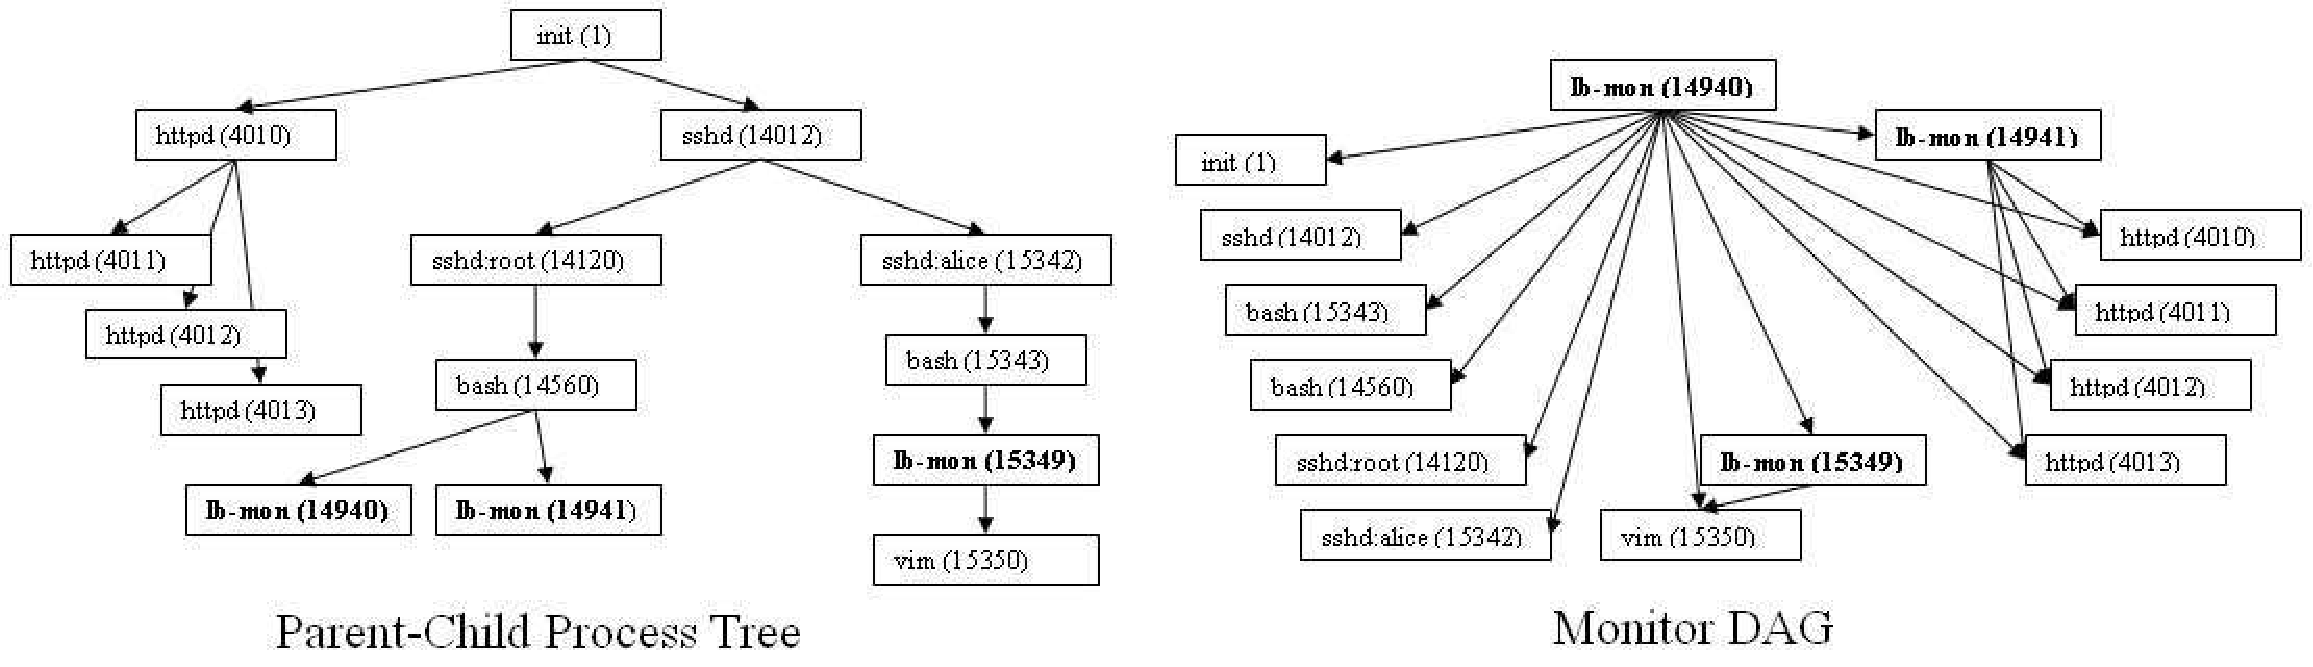
\includegraphics[scale=0.4]{lbox-mon-both}
\caption{A Tree of Cascaded Monitors}
\label{mon-tree}
\end{figure*}


% While a simple example was used, it should be clear that only
% a fairly minimal kernel mechanism which is attached
% to relevant actions and objects is needed.
% The monitor process can pretty much do anything. 
% LAFS \cite{lafs}
% is a logging and auditing file system where accesses not conforming
% to a policy are logged.
% The policy specification
% includes a time interval, userid specification, application
% and operation type. A LAFS-like monitor could easily be written.
% While file events do not specify the application issuing the operation,
% the monitor can reconstruct this from the {\tt execve} events.
% Note that it is harder to use {\tt DTrace} to do this LAFS-style tracing 
% because of its system call orientation. Here we can make use of 
% inheritance in the directory structure. 
% A related but slightly simpler monitor is to audit whether
% the apache web server is used to access any unexpected files.

% In \cite{finke} a monitoring application is described to report when 
% applications tasks did not run as they were supposed to, e.g. due to some
% failure. Again, it is easy to write a monitor which can detect whether
% tasks ran as scheduled.

%% can add application events

\subsection{Using Monitors}

We now give some simple examples of using the framework.
This examples are only meant to exemplify the ease of creating
a customized auditing monitor and are not meant to be full blown applications.

\subsubsection{Testing a possibly untrusted program}

This example checks to see if a process is not stealing your PGP keys.
The monitor process first creates the lbox and then a child process
which executes the program to be audited.

{
\small
\begin{verbatim}
  proc_spec = lbox_CHILDOF(getpid());
  lbox_addevent_file(event_spec,
    "/home/alice/.gnupg/secring.gpg",
    SELF, F_R, I_ALL);
  // .... create the lbox
  if (fork()) {
          // .... do the event processing
  } else execl(....);
\end{verbatim}
}

% The process specification is described by all the child processes 
% of the monitor.
% This makes sure there is no race condition between monitor
% creation time and child process execution time.
% Note that the monitor never monitors itself,
% because it will create a monitoring cycle.
% It is automatically removed from the set of monitored processes.


\subsubsection{Monitoring the web server}

In this example, we want to see whether the web server is working correctly.
More precisely, we want to make sure it is only accessing files inside
\code{/var/www}.

The process specification can be described as follows:
{
\small
\begin{verbatim}
  proc_spec = lbox_CHILDOF(apach_master_pid);
\end{verbatim}
}
\noindent
The event specification is an example of
monitoring files {\em outside} some directory.
We first make all files to be monitored, then we make
all files under \code{/var/www} {\em not} to be monitored.
Note that the order of the two specifications is not important.
{
\small
\begin{verbatim}
  lbox_add_event_file(&event_spec1, "/",
    SELF|SUBDIRECTORIES, F_R|F_W, I_ALL);
  lbox_add_event_file(&event_spec2,
    "/var/www", IGNORE, F_R|F_W, I_ALL);
\end{verbatim}
}
% In the first event specification,
% we make all files to be monitored by issuing the root
% directory and its subdirectory to be monitored.
% In the second event specification,
% we get rid of \code{/var/www} by using IGNORE as the
% directory inheritance flag.

\subsubsection{Global Monitoring}

Sometimes you need to monitor all actions on a single process;
and other times you need to monitor a single action on all processes.
In this example, we want to see if any process is sending packets
to the network \code{137.132.0.0/255.255.0.0}.
The process specification is simply, \\
{\small\verb|  proc_spec = lbox_TRUE();|} \\
The event specification is the following network event, \\
{\small\verb|  lbox_net_connect_ipv4(&event_spec,|} \\
{\small\verb|    "137.132.0.0/255.255.0.0");|}

\subsubsection{Other Applications}

LAFS \cite{lafs}
is a logging and auditing file system where accesses not conforming
to a policy are logged.
The policy specification
includes a time interval, userid specification, application
and operation type. A LAFS-like monitor could easily be written.
Note that it is harder to use {\tt dtrace} to do this LAFS-style tracing 
because of its system call orientation. Here we can make use of 
inheritance in the directory structure. 

In \cite{finke} a monitoring application is described to report when 
applications tasks did not run as they were supposed to, e.g. due to some
failure. Again, it is easy to write a monitor which can detect whether
tasks ran as scheduled.

% \subsection{Implementation Issues}
% 
% \subsubsection{The Hooking Mechanism}
% 
% The prototype implementation we have is in Linux on the 2.6 kernel series.
% There are several ways of implementing the monitor mechanism:
% \begin{enumerate}
% \item Making use of the {\tt ptrace()} or {\tt /proc} facility.
% As discussed earlier, this has many problems and does not support
% mandatory or reliable monitoring. A system-call based mechanism
% is also not suitable for our object-based orientation.
% \item Some other in-kernel system call interposition method.
% This can suffer from TOCTOU (time of create time of use) problems.
% For example, if we are monitoring the {\tt write()} system call,
% a process can change the actual file which the file descriptor points to
% between the time when the file descriptor is looked up and 
% the actual file descriptor is used.
% This would lead either to missing an event (unreliability) or
% reporting an incorrect event (the wrong file).
% As before, it also does not suit our object-based orientation.
% \item Using the LSM hooks in Linux 2.6.
% We currently use this approach in our prototype which has a good
% match with kernel objects. Its also much simpler as LSM hooks are
% mostly in the right places.
% It guarantees mandatory monitoring, and does not suffer from TOCTOU.
% However, it does not cover every possible system calls.
% As the present prototype focuses initially on events on files,
% this is sufficient but it does mean that a full solution cannot be
% just a module.
% \end{enumerate}
% 
% \subsubsection{Matching The File Specification}
% 
% Matching file event specifications, requires the 
% deeper matching file event specification to take precedence.
% To achieve this, the algorithm for checking of a file access is as follows.
% \begin{enumerate}
% \item If the current file is marked SELF, report it (generate event), done.
% \item If the current file is marked SUBDIRECTORIES, report it (generate event), done.
% \item If the current file is marked IGNORE (neither SELF nor SUBDIRECTORIES), ignore it,
% done.
% \item If it is the root directory, ignore it, done.
% \item Set parent directory as current file.
% \item Goto 2.
% \end{enumerate}
% 
% Suppose we have the following two file event specifications
% from the previous example:
% \begin{enumerate}
% \item {\tt (/, SELF|SUBDIRECTORIES, R|W)}
% \item {\tt (/var/www, IGNORE, R|W)}
% \end{enumerate}
% For the file /var/www/a/b/c, the checking is stopped
% at {\tt /var/www} at the third step.
% For the file /etc/passwd, the checking is stopped
% at {\tt /} at the second step.
% 
% To do the upward directory traversal, we make use of the
% {\tt dentry} kernel structure.
% The upward directory traversal is fast, because in Linux,
% during the path resolving phase, all the parent {\tt dentry}
% nodes are stored in the {\tt dcache}.
% 
% \subsubsection{Performance Tuning Methods}
% 
% To reduce the overhead of of task switching caused by our auditing system,
% we introduce an event buffer so that the monitored process 
% can continue its execution even if it generates a auditing event.
% Timeouts and events with a flushing property
% are used to ensure that the monitor can still get events
% even if the buffer is not full and the monitor can choose
% a tradeoff between efficiency and timeliness.
% 
% When a system call takes place, we first check whether the process is being
% monitored.
% This check only requires a few instructions.
% Thus there is very little impact on non-monitored processes.
% For monitored processes, the monitor can also be found efficiently.
% Thus there is very little impact on a process as long as
% the number of logboxes which contains the process is not too large.
% 
% The time required for checking whether the event should be logged
% varies with different types of events.
% A direct operation involving the file is very efficient.
% If there is any file event which involves inheritance,
% we need to trace the file all the way up to the marked file 
% or the root directory.
% Since all the information of parent files is in the dentry cache,
% the directory traversal should be fast.
% Other kinds of objects can be equally fast, for example,
% with a socket connection event, we only need to do the netmask test.

\subsection{Experimental Evaluation}

Our prototype Linux implementation makes use of LSM \cite{lsm} and
version 2.6.10 of the kernel,
and thus is convenient to install
as it consists of loadable kernel modules.
The interface to the kernel is done through \code{ioctl} to a pseudo filesystem
in \code{/proc/lbox}.
The lbox API library in Section \ref{sec:framework} 
gives a more convenient interface that using \code{ioctl} system calls.
Due to lack of space, we do not go into further details
of the kernel implementation.
The PC used here is a Pentium IV 3.0GHz PC with 1G memory.

We want to demonstrate that the framework and prototype system leads
to rather efficient monitoring. Although our prototype is not yet
fully optimized, the results do show that the overheads of monitoring
can be very low.

We first use a simple micro-benchmark which gives an indication
of worse case overheads.
The program performs 1000000 open(2) and close(2) calls with
a monitor watching for the file access.
We compare the auditing framework in each of the following scenarios:
\begin{enumerate}

\item {\em clean kernel}:
A clean stock kernel.

\item {\em proc miss}:
The lbox module is loaded in the kernel but no monitors are present.
% However, no monitor is monitoring the busy-open process.

\item {\em file miss 1/2}:
A monitor is monitoring the file open but on a different file specification.
Thus no event is generated.
We compare two scenarios.
{\em File miss 1}, uses a directory specification without the
SUBDIRECTORIES property, thus no directory traversal is needed.
{\em File miss 2} has a file specification which is some non-matching
directory with the SUBDIRECTORIES set.
This requires traversing up ancestor directories up to the root.
% check whether the event can match the directory specification.
% The difference between the two scenarios is whether directory traversal
% is needed. 
% SUBDIRECTORIES flag set, whereas in {\em file miss 2}, there is a file spec
% which has SUBDIRECTORIES flag set, thus we need to traverse all the way up to
% the root directory to make sure that the action does not match the file spec.

\item {\em 0 dir level}:
The monitor is monitoring a regular file.
The benchmark is accessing the same regular file.

\item {\em 1/2 dir levels}:
The monitor is monitoring a directory which is 1 or 2 levels deep containing
the which is being used.
For example, the monitor uses the file specification
\code{/1} with SUBDIRECTORIES set.
The 2 dir level benchmark opens the file \code{/1/2/foo}.
This test investigates the time for directory traversal..

\item {\em no buff}:
The file event is synchronous which means 1000000 context switches
to the monitor are needed.
The benchmark process suspends until the monitor
has read the event

\item {\em ptrace}:
The comparison is with \code{strace} which uses the traditional
\code{ptrace} mechanism in Linux.

\end{enumerate}

\begin{table}
\small
%\begin{center}
\centering
\begin{tabular}{ | l || c | c | c | }
\hline
scenario & real & user & sys \\
\hline \hline
clean kernel & \begin{math} 1.99\pm0.01 \end{math} & \begin{math} 0.21\pm0.01 \end{math} & \begin{math} 1.77\pm0.02 \end{math} \\
proc miss & \begin{math} 2.04\pm0.02 \end{math} & \begin{math} 0.21\pm0.01 \end{math} & \begin{math} 1.82\pm0.03 \end{math} \\
file miss 1 & \begin{math} 2.17\pm0.01 \end{math} & \begin{math} 0.22\pm0.01 \end{math} & \begin{math} 1.95\pm0.02 \end{math} \\
file miss 2 & \begin{math} 2.27\pm0.01 \end{math} & \begin{math} 0.22\pm0.01 \end{math} & \begin{math} 2.04\pm0.02 \end{math} \\
1 dir level & \begin{math} 2.29\pm0.01 \end{math} & \begin{math} 0.21\pm0.01 \end{math} & \begin{math} 2.03\pm0.02 \end{math} \\
2 dir levels & \begin{math} 2.52\pm0.01 \end{math} & \begin{math} 0.21\pm0.01 \end{math} & \begin{math} 2.23\pm0.03 \end{math} \\
3 dir levels & \begin{math} 2.56\pm0.01 \end{math} & \begin{math} 0.20\pm0.02 \end{math} & \begin{math} 2.31\pm0.02 \end{math} \\
no buff & \begin{math} 8.70\pm0.04 \end{math} & \begin{math} 0.99\pm0.08 \end{math} & \begin{math} 4.57\pm0.16 \end{math} \\
ptrace & \begin{math} 59.04\pm0.15 \end{math} & \begin{math} 12.90\pm0.32 \end{math} & \begin{math} 46.11\pm0.39 \end{math} \\
\hline
\end{tabular}
%\end{center}
\caption{Open micro-benchmark}
\label{tab-open}
\end{table}

The open micro-benchmark results are given in Table \ref{tab-open}
with all times in seconds. The average and standard deviation
is given over 10 runs.
As the timings are only measured with the Unix user/system and real-time
mechanism, they are only approximate and are meant
to give an indication of the overheads of monitoring
under the different scenarios.

The kernel inspection implementation (proc miss) has negligible overhead
($\sim 2\%$) over the clean kernel.
The {\em file miss 2} test has ($\sim 14\%$) overhead, this is because that
the system needs to travel to the root directory to make sure the file is
not monitored.
{\em file miss 1} has a smaller overhead ($\sim 9\%$) because directory
traversal is not needed.
When monitoring is synchronous, so events are not buffered (no buff),
overhead jumps substantially to $337\%$.
It is interesting to note that this is still much smaller than {\tt ptrace}
which has $2866\%$ overhead or about seven times slower than the
no buffering case.
Using asynchronous events with buffering (0 dir level) 
drops the overhead to $15\%$.

One point of comparison with other systems on Linux would be with
Systrace \cite{systrace}. 
A pure comparison is not valid since in our system any event
which must be monitored is eventually passed to the monitor.
Systrace on the other as it does access control first can choose between a
kernel-level policy or the user-level policy daemon. 
The kernel-level policy should entail less work for Systrace
simply because the decision is handled only within the kernel, while
the user-level policy is more expensive simply due to the increased
number of context switches.
The objectives of the two systems are also different.
With those caveats in mind, the Systrace open micro-benchmark shows a
$6.25\%$ overhead over no monitoring.
Our overhead for {\em file miss 1} is a little more at $9\%$.
This makes sense since for auditing,
an event has to cross in two directions: first inwards when it is recorded; 
and later back to user-space when it is sent to the monitor.
Our implementation is not yet optimized and we expect also to be
able to reduce the overheads further.

Our directory file specifications can be compared against the 
pathname normalization of Systrace.
The ``0-2 dir levels'' scenario shows that the overhead of an inherited
file specification is small, the initial overhead of checking a directory is
reasonable at $26\%$ and then a rather small overhead for the next component.
The Systrace results show that each directory
component in their specification adds about $1665\%$ additional overhead
over the original {\tt open()} system call.
This is because of the filename normalization done in user-space which
is significantly more expensive.

\begin{table}
\small
%\begin{center}
\centering
\begin{tabular}{|l||c|c|c|}
\hline
scenario & real & user & sys \\
\hline \hline
direct run & \begin{math} 3.84\pm0.01 \end{math} & \begin{math} 1.04\pm0.01 \end{math} & \begin{math} 2.80\pm0.01 \end{math} \\
\hline
truss & \begin{math} 100.32\pm0.85 \end{math} & \begin{math} 10.12\pm0.05 \end{math} & \begin{math} 56.71\pm0.80 \end{math} \\
\hline
DTrace\footnotemark & \begin{math} 8.41\pm0.02 \end{math} & \begin{math} 1.08\pm0.01 \end{math} & \begin{math} 7.33\pm0.01 \end{math} \\
\hline
\end{tabular}
%\end{center}
\caption{Open micro-benchmark on Solaris 10}
% (SunOS 5.10 i386)}
\label{tab-sol}
\end{table}

\footnotetext[2]{The D program is ``syscall::open:entry \{ @[execname]=count(); \}''}

Table \ref{tab-sol} shows the
test on Solaris for the same hardware with the same benchmark program. 
While the baseline for Solaris is slower than Linux, it is reasonable
to make relative comparisons.
\code{Truss} which uses the \code{proc} adds $2510\%$ overhead 
to the \code{open()} system call and DTrace is significantly more efficient
with $119\%$ overhead.
The use of \code{proc} allows only the \code{open()} system call to
be traced rather than all system calls. Even so, we see that the overhead
is considerably higher than in Linux where \code{ptrace} traces every
system call.
In the DTrace test, we have allowed DTrace more advantage 
as the D program does not return any information to user space, 
whereas in our system, all
the relevant {\tt open()}'s are being
returned to the user space monitor.
The absolute running time in the DTrace test is 3.67 times 
of that in our system.
The overhead added to the original system call in DTrace is 7.9 times of
that in our system.
This is slightly surprising since DTrace uses dynamic instrumentation
(which is hardware dependent) while we use a simpler static instrumentation
which is more expensive but portable.
We suspect it is partly a case of the Linux kernel having less overhead
than Solaris.

% Since the open micro-benchmark reuses the same file over and over again,
% the open itself becomes quite fast in Linux. 
% We use another micro-benchmark on socket
% operations to show the effect of a more expensive system call.
% The benchmark creates a TCP socket and connects to a local port.
% This is repeated for 4000 times and the results are in Table \ref{tab-connect}.
% We can see that in an expensive system call, the overhead is not noticeable.

% \begin{table}
% %\begin{center}
% \centering
% \begin{tabular}{ | l || c | c | c | }
% \hline
% environment & real & user & sys \\
% \hline\hline
% clean kernel & \begin{math} 0.27\pm0.01 \end{math} & \begin{math} 0.01\pm0.01 \end{math} & \begin{math} 0.20\pm0.01 \end{math} \\
% \hline
% monitored & \begin{math} 0.28\pm0.01 \end{math} & \begin{math} 0.01\pm0.01 \end{math} & \begin{math} 0.20\pm0.01 \end{math} \\
% \hline
% \end{tabular}
% %\end{center}
% \caption{Connect micro-benchmark}
% \label{tab-connect}
% \end{table}

\begin{table*}[ht]
\centering
\begin{tabular}{ | l || c | c | c | }
\hline
 & web server (request/sec) & make bash (sec) & install mozilla (sec) \\
\hline\hline
Linux clean & \begin{math} 8903.1\pm21.8 \end{math} & \begin{math} 34.3\pm0.2 \end{math} & \begin{math} 1.8\pm0.1 \end{math} \\
\hline
lbox no I/O, file miss & \begin{math} 8773.1\pm19.4 (1.5\%) \end{math} & \begin{math} 34.4\pm0.2 (0.17\%) \end{math} & \begin{math} 1.8\pm0.0 (0\%) \end{math} \\
\hline
lbox no I/O, file hit & \begin{math} 8762.0\pm25.6 (1.6\%) \end{math} & \begin{math} 34.4\pm0.2 (0.17\%) \end{math} & \begin{math} 1.8\pm0.0 (0.56\%) \end{math} \\
\hline
lbox with I/O & \begin{math} 8728.9\pm18.4 (2.0\%) \end{math} & \begin{math} 34.4\pm0.2 (0.29\%) \end{math} & \begin{math} 1.7\pm0.1 (3.9\%) \end{math} \\
\hline
strace no I/O & \begin{math} 3577.6\pm8.5 (148.9\%) \end{math} & \begin{math} 39.6\pm0.1 (15.3\%) \end{math} & \begin{math} 2.2\pm0.1 (21.1\%) \end{math} \\
\hline
strace with I/O & \begin{math} 1981.4\pm6.9 (349.3\%) \end{math} & \begin{math} 100.7\pm0.1 (293.2\%) \end{math} & \begin{math} 23.2\pm0.1 (1189.4\%) \end{math} \\
\hline\hline
Solaris clean & \begin{math} 6889.1\pm42.6 \end{math} & \begin{math} 43.8\pm0.1 \end{math} & \begin{math} 1.6\pm0.1 \end{math} \\
\hline
DTrace no I/O & \begin{math} 6776.2\pm53.6 (1.7\%) \end{math} & \begin{math} 44.4\pm0.1 (1.4\%) \end{math} & \begin{math} 1.6\pm0.1 (0\%) \end{math} \\
\hline
DTrace with I/O & \begin{math} 6326.9\pm52.4 (8.9\%) \end{math} & \begin{math} 44.5\pm0.0 (1.6\%) \end{math} & \begin{math} 1.6\pm0.0 (0.6\%) \end{math} \\
\hline
truss no I/O & \begin{math} 1382.0\pm2.0 (398.5\%) \end{math} & \begin{math} 70.9\pm0.0 (61.8\%) \end{math} & \begin{math} 7.7\pm0.0 (372.2\%) \end{math} \\
\hline
truss with I/O & \begin{math} 1126.7\pm4.4 (511.5\%) \end{math} & \begin{math} 74.6\pm1.5 (70.2\%) \end{math} & \begin{math} 13.4\pm0.13 (724.7\%) \end{math} \\
\hline
\end{tabular}
\caption{Macro-benchmarks}
\label{tab-macro}
\end{table*}

The \code{open} micro-benchmark gives a measure of worst-case overhead
since the file is totally cached in memory and in that case, the Linux
\code{open} code is heavily optimized.
It is also useful to look at applications (macro-benchmarks
which do more than just system calls) which may have moderate to
moderately heavy system call usage. Obviously, there is little point
benchmarking CPU bound applications which only have low system call use.
In the macro-benchmarks, we also look at the cost of monitoring 
I/O (reading and writing), this is meant to simulate a monitor which might
want to examine precisely what an application has done.
We have chosen three application benchmarks which are realistic applications
\begin{itemize}
\item apache web server: this is chosen because web server performance
is important.
For apache, we measure the average number of requests served per second
using the apache \code{ab} benchmark and I/O monitoring is for
the http requests (reading) and http responses (writing).

\item \code{make bash}: this builds the bash shell.

\item install mozilla: this installs mozilla. The
Linux and Solaris differ. The Linux one has a custom
install program while the Solaris version is simply untar.
This means the results are not comparable except in a relative
to each operating system alone.
\end{itemize}

The last two benchmarks, bash and mozilla,
have also been chosen because these applications
have been used in Alcatraz.
For I/O monitoring, we have monitored all the I/O from the application.
The results given in Table \ref{tab-macro}. 
The results for \code{strace} and \code{truss} are only meant to illustrate
the additional overhead of I/O since both programs do reprocess the data
and thus do have additional overhead but 
serves to bound the cost of \code{ptrace} and \code{proc}.
We see that in all cases, lbox monitoring has very low overheads, below
$2\%$ without I/O and less than $4\%$ with complete I/O monitoring of the
applications.
The mozilla install cannot be directly compared since the actual install
is different.
Even though these are macro-benchmarks, 
overhead for \code{ptrace} without I/O is significant, at least $15\%$.
With I/O monitoring, the overhead shoots up.
Alcatraz \cite{alcatraz} which uses \code{ptrace} has rather
high overheads for their system call interception, $43\%$ for a \code{make}
and $79\%$ for \code{mozilla}. Their isolation overhead which is a measure
of write I/O adds a further $20\%$. Our overheads are much smaller ($< 4\%$)
but we don't do isolation.

It is a little surprising that our user-level auditing framework
can out perform DTrace which is an in-kernel tracing mechanism.
This is very encouraging and furthermore, 
we believe we can still optimize our prototype.

\subsection{Conclusion}

We show a user-level auditing framework suitable for general purpose
auditing and security monitoring. 
We achieve transparent auditing
at a fine-grained level of applications while providing guarantees
on the security of the auditing process. We are careful to avoid problems
with privilege escalation and access to information beyong the user's
privileges. Furthermore, we avoid problems associated with denial of
service which can be caused by self-referential monitoring or tracing.

As our monitors are user-level, the auditing is expressed in terms
of operations on operating system objects and resources. This makes it
easy to write a custom monitor since the semantics is close to that
of user code rather than having to understand kernel internals.

A user-level monitor is desirable given it is more safe than an in-kernel one.
The question is whether a user-level monitor is sufficiently efficient. 
Our framework is designed so that the cost of monitoring
is commensurate with the amount of events and information needed.
Our experiments are very encouraging 
showing that the overhead is comparable to in-kernel 
mechanisms such as DTrace.

Future work includes further system optimizations to make the framework
even more scalable and efficient. We would like to increase the
expressivity of the in-kernel mechanisms without incurring more cost
and also avoiding executing monitor code in the kernel.

% \begin{thebibliography}{99}
% 
% \bibitem{dtrace-paper}
% Bryan M. Cantrill, Michael W. Shapiro and Adam H. Leventhal,
% ``Dynamic Instrumentation of Production Systems'',
% Usenix, 2004.
% 
% \bibitem{finke}
% J. Finke,
% ``Process Monitor: Detecting Events That Didn't Happen'',
% Usenix LISA, 2002.
% 
% \bibitem{garfinkel}
% T. Garfinkel,
% ``Traps and Pitfalls: Practical Problems in System Call 
% Interposition Based Security Tools'',
% Network and Distributed Systems Security Symp,
% 2003.
% 
% \bibitem{janus}
% I. Goldberg, D. Wagner, R. Thomas, and E. Brewer,
% ``A Secure Environment for Untrusted Helper Applications'',
% Usenix Security, 1996.
% 
% \bibitem{alcatraz}
% Z. Liang, V.N. Venkatakrishnan, and R. Sekar, 
% ``Isolated Program Execution: An Application
% Transparent Approach for Executing Untrusted Programs'',
% ACSAC, 2003.
% 
% \bibitem{systrace}
% N. Provos,
% ``Improving Host Security with System Call Policies'',
% Usenix Security, 2003.
% 
% \bibitem{solaris-sec-svc}
% Sun Microsystems,
% ``System Administration Guide: Security Services'',
% part IV: Auditing and Device Management.
% 
% % \bibitem{dtrace-man}
% % Sun Microsystems,
% % ``Solaris Dynamic Tracing Guide''.
% 
% \bibitem{lafs}
% C. Wee,
% ``LAFS: A Logging and Auditing File System'',
% Annual Computer Security Applications Conf,
% 231--240, 1995.
% 
% \bibitem{lsm}
% C. Wright, C. Cowan, S. Smalley, J. Morris, and G. Kroah-Hartman,
% ``Linux Security Modules: General Security Support for the Linux Kernel'',
% Usenix Security, 2002.
% 
% \bibitem{dprobes}
% Dynamic Probes,
% {\small\tt http://dprobes.sourceforge.net/}
% 
% \end{thebibliography}
% 
% \end{document}
